%!TEX root = main-ugly.tex
We applied the robust controller synthesis of \S \ref{sec:robust-perf} to the scaled doubly-stochastic chain system\footnote{All code needed to reproduce examples in this section can be found at \url{https://github.com/nikolaimatni/robust-sls}.}:
\begin{equation}\label{eq:chain}
\begin{array}{rcl}
x^1_{t+1} &=& \rho\left[(1-\alpha)x^1_t + \alpha x^2_t\right] + u^1_t\\
x^i_{t+1} &=& \rho\left[\alpha x^{i-1}_t + (1-2\alpha)x^i_t + \alpha x^{i+1}_t\right] + u^i_t,\\
&& \text{ for $i=2,\dots,N-1$,} \\
 x^N_{t+1} &=& \rho\left[\alpha x^{N-1}_t + (1-\alpha)x^N_t\right] + u^N_t
 \end{array}
\end{equation}
where the $x^i_t, u^i_t \in \R$ are the scalar state and inputs, respectively, of the subsystems, and we set the number of scalar subsystems $N=50$, the scaling factor $\rho = 0.5$, and the coupling constant $\alpha = 0.49$.  

We solve the robust performance performance problem \eqref{eq:constraints} under both centralized and localized distributed constraints. We assume the the uncertainty to be norm-bounded by $\epsilon = 0.55$. We fix cost matrices $C^\top = [I_N, 0]$ and $D^\top = [0, 5I_N]$.  For both settings, we impose a FIR horizon of $T=10$ when solving the robust performance problem \eqref{eq:constraints}.  Additionally, we enforce that the corresponding system responses satisfy $d$-locality constraints -- intuitively, these constraints ensure that in closed loop, the disturbance striking node $i$ only affects nodes $j$ satisfying $|j-i|\leq d$. A smaller $d$ corresponds to a more localized closed loop response.\footnote{In the interest of clarity, we do not enforce communication delay constraints, but note that both communication delay and locality constraints can be enforced through suitable sparsity constraints on the system response variables: see \cite{anderson2019system} for details.}

By bisecting on $\gamma$, we determine that the optimal robust performance level is $\gamma = 5.57$ for both centralized and distributed controllers, where for the distributed controller we set the locality diameter to $d=2$.  That there is no gap between centralized and distributed is not surprising because: (i) we impose no communication delay constraints, and (ii) $\mathcal{L}_1$ optimal control leads to deadbeat closed loop responses, which will consequently also be localized.  The nominal $\mathcal{L}_1$ norms  (i.e., performance on system with no uncertainty) of the closed loop systems for the centralized and distributed localized robust controllers are both $2.5$, while the norms achieved by the optimal $\mathcal{L}_1$ controllers (i.e., without robustness constraints) are $1.43$ and $2.47$, respectively.  Notice that there is an appreciable degradation in nominal performance in the centralized setting, but not in the localized distributed setting.  We conjecture that this is due to the sparsity of the augmented plant $\tf M$ defined by the system response $\Phih$, which constrains both robust and nominal systems to behave similarly.

To test this conjecture, we examine the relationship of the closed loop norm of the robust and optimal controllers to perturbations of the form $\DA = \mathrm{blkdiag}(\kappa I, \kappa I, \dots)$ and $\DB = 0$, for $\kappa \in [0,\epsilon]$, for locality parameters $d\in\{2,5\}$; results for larger $d$ are indistinguishable from the centralized setting. The results are displayed in Fig \ref{fig:kappa}.  When $d=5$, the robust controller enjoys improved performance for larger values of $\kappa$, at the expense of degraded performance at lower values. By contrast, in the ``extremely'' localized setting of $d=2$, the degrees of freedom are limited such that robust and nominal control behave similarly.  

We also examine the closed loop responses computed for the centralized and localized ($d=2$) controllers, with and without robustness constraints. Although the closed loop map is constrained to an FIR horizon of $T=10$, the addition of robustness constraints in the centralized case shortens the impulse response horizon such that $\Phih_x \approx I$. Intuitively, disturbances are allowed to persist in the nominal centralized case, but not in the robust centralized case. In the localized setting, the nominal controller has shortened horizons, and again is not noticeably different from the robust controller. These observations motivate future work, highlighting that our approach allows for a principled exploration of tradeoffs between complexity of synthesis and implementation (as measured by $d$), nominal performance, and robust performance for large-scale distributed systems.

\begin{figure}
\centering
~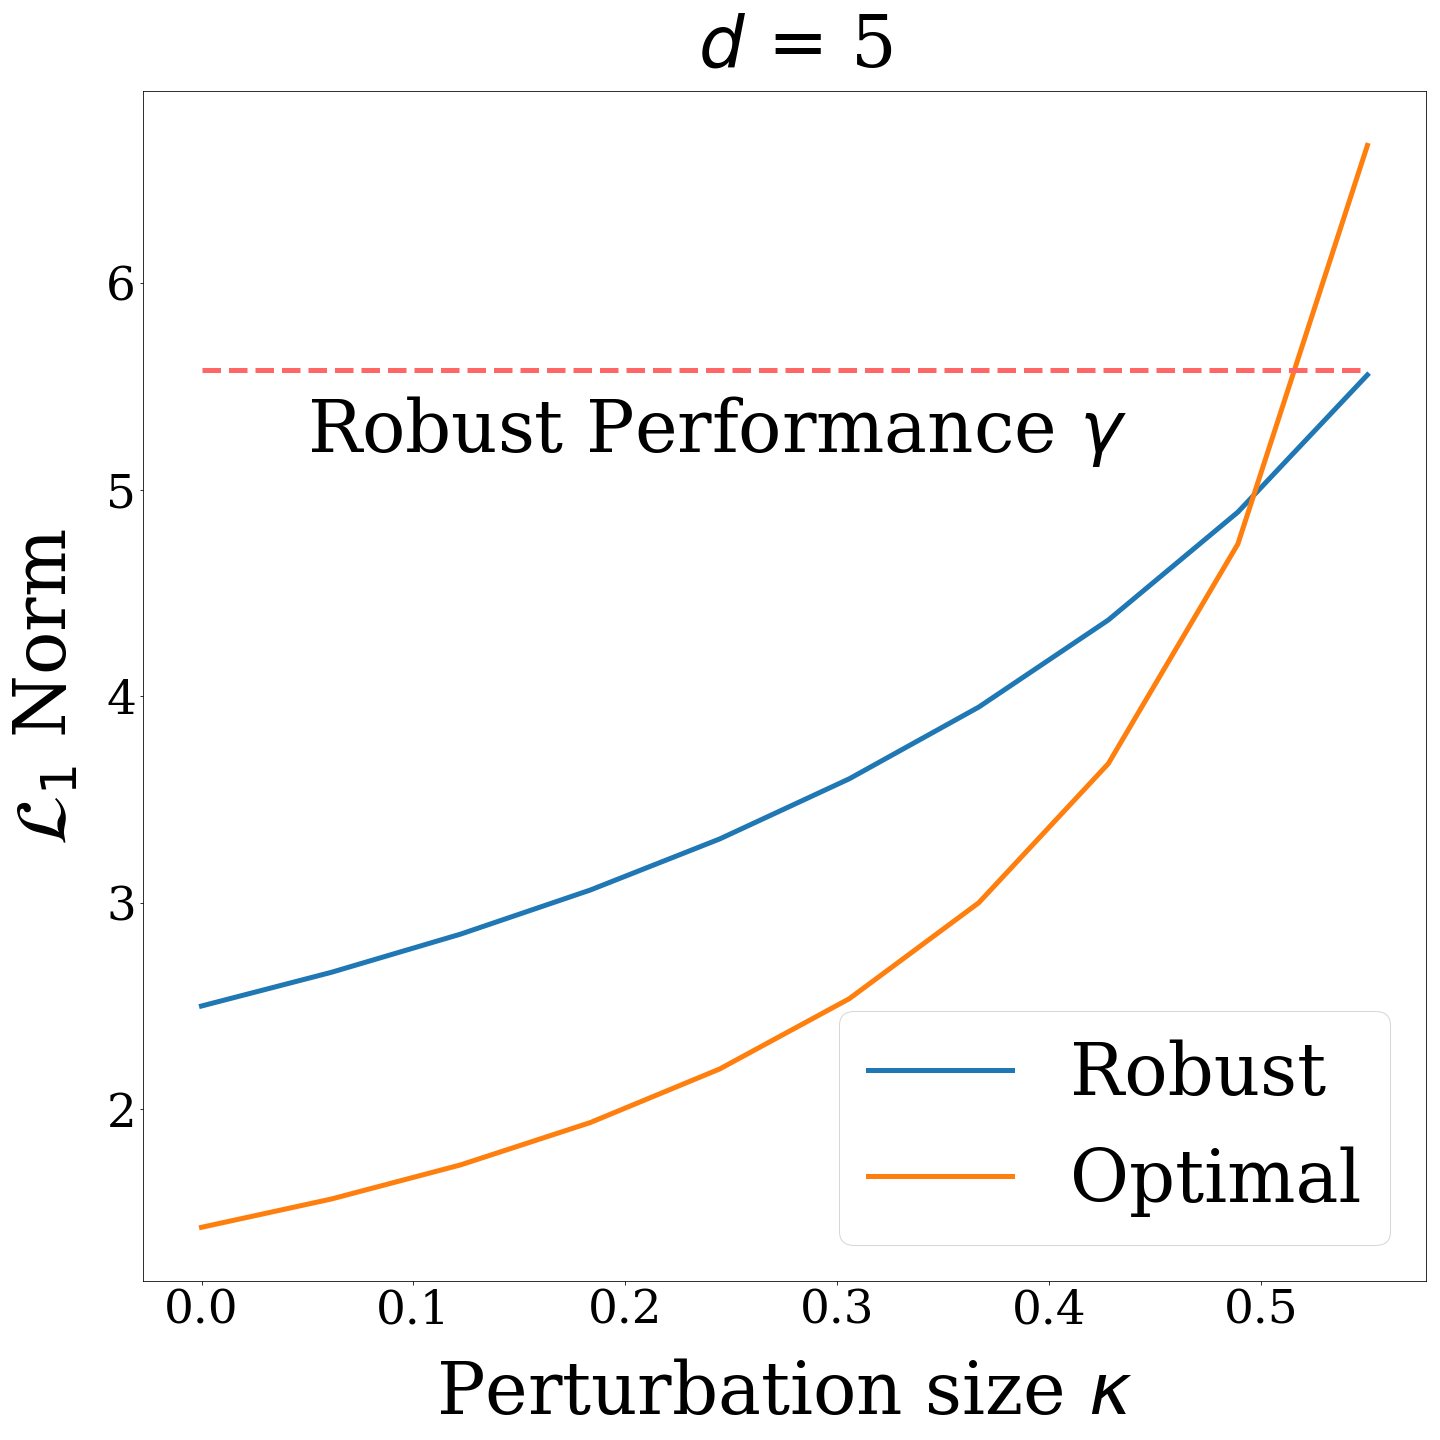
\includegraphics[width=.45\columnwidth]{d5.png}~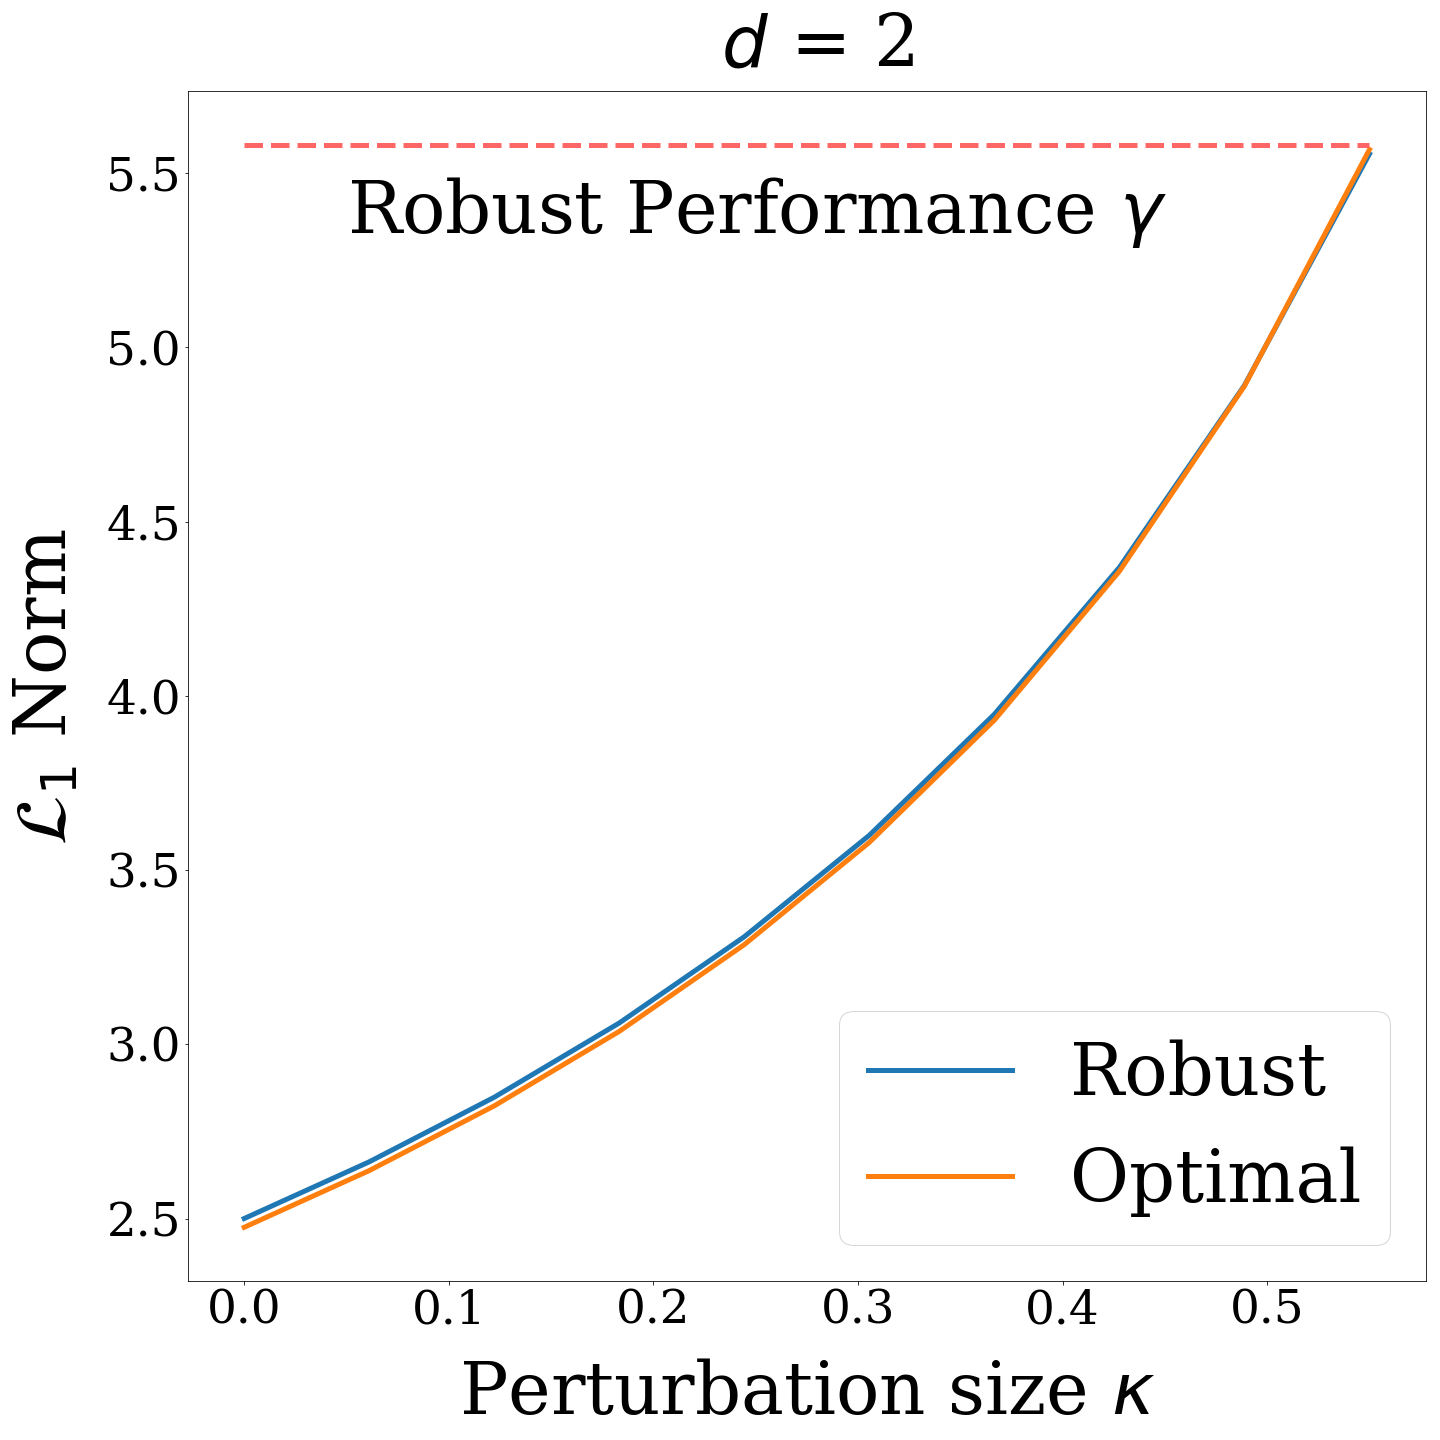
\includegraphics[width=.45\columnwidth]{d2.png}~
\caption{Performance of robust \& optimal controllers, with uncertainty  $\DA = \mathrm{blkdiag}(\kappa I, \kappa I, \dots)$, $\DB = 0$. }%As $\kappa$ increases to $\epsilon = 0.55$, performance of the robust controller meets the robust performance bound $\gamma$ \eqref{eq:constraints}.}
\label{fig:kappa}
\end{figure}

%Finally we note that even without exploiting any of the underlying partial separability of the resulting problem (see \cite{wang2018separable}), we are able to solve the resulting centralized and distributed localized feasibility problems \eqref{eq:constraints} in 29s and 114s,\footnote{The majority of this time was spent on pre-processing by MOSEK: the actual solve time required by the optimizer was under 1s.} respectively, on a 2.3GHz 8 Core MacBook Pro with 32 GB of RAM using CVXPY \cite{diamond2016cvxpy} and MOSEK \cite{andersen2000mosek}.